\documentclass[compress]{beamer}

\usepackage{lmodern}
\usepackage{hyperref}
\usepackage{graphicx}
\usepackage{minted}
\usepackage{epstopdf}
\usepackage{ulem}

\title{Git gud \texttt{--fast-forward}}
\subtitle{Git voor beginners}
\author{Sticky: CommIT}
\date{30 november 2016}

\usetheme{Frankfurt}
\usecolortheme{dove}

\setbeamertemplate{section in toc}{\inserttocsectionnumber.~\inserttocsection}
\setbeamertemplate{itemize items}[default]
\setbeamertemplate{enumerate items}[default]

% ToC invoegen aan het begin van elke sectie.
\AtBeginSection
{
  \begin{frame}
      \tableofcontents[currentsection,hideallsubsections,subsubsectionstyle=hide]
    \end{frame}
}
% Bron: https://en.wikibooks.org/wiki/LaTeX/Presentations

\definecolor{light-gray}{gray}{0.90}

\begin{document}

\frame{\titlepage
	\begin{center}
		Slides: \url{http://j.mp/gitgudslides} (\texttt{main.pdf})
	\end{center}
}

\section[W\&H?]{Waarom \& hoe git?}

\subsection{Version control}
\begin{frame}{Wat is version control?}
	Op een niet-onhandige manier:
		\begin{itemize}
			\item Code delen met meerdere mensen
			\item Geschiedenis bijhouden / terugdraaien
			\item Veranderingen (evt. over langere tijd) zichtbaar maken
			\item Overzicht van wie wat veranderde
		\end{itemize}
\end{frame}

\subsection{Waarom git?}
\begin{frame}{Waarom git?}
	\begin{itemize}
		\item Distributed:
			\begin{itemize}
				\item Je hebt zelf (standaard) de gehele geschiedenis
				\item Je kan zonder internet werken
			\end{itemize}
		\item Integrity: bestanden kunnen niet veranderen zonder dat git het merkt
		\item Moeilijk om data te vernietigen (`kwijt' kan maar dan moet je beter opletten)
		\item Non-lineair: kan veel dingen naast elkaar starten (en weer weggooien)
		\item Veel diensten op gebouwd: Github, Travis, \ldots
	\end{itemize}
\end{frame}

\begin{frame}{Waarom command line?}
	\begin{itemize}
		\item Hetzelfde over alle platforms
		\item GUIs gebruiken zelfde namen voor dingen
		\item GUI gaat kapot: `ja ga maar command line'
		\item Meer hulpmogelijkheden: \texttt{git help}
	\end{itemize}
	Goede GUIs: zie \href{https://git-scm.com/downloads/guis}{de site van git}
	\begin{itemize}
		\item SmartGit \url{https://syntevo.com/smartgit/} (niet-vrij)
		\item Gitkraken \url{https://gitkraken.com} (niet-vrij)
	\end{itemize}
	Als je de command line snapt, snap je de andere clients!
\end{frame}

\section[Structuur]{Structuur van Git}
\subsection{DAG}
\begin{frame}{Graaf}
	Git gebruikt een \emph{Directed Acyclic Graph}/ gerichte acyclische graaf:
	\begin{itemize}
		\item Eindig veel bolletjes: \emph{commits}
		\item Bolletjes wijzen naar hun voorganger, maar niet andersom
		\item Er kunnen geen loops inzitten
		\item Verwijzingen naar de commits: \emph{refs}
	\end{itemize}

	\begin{center}
		\includegraphics[width=.6\textwidth]{graphs/dagview.eps}
	\end{center}
\end{frame}

\subsection{Locaties}
\begin{frame}
	3 plekken waar je gegevens zitten:\\
	\vspace{.5cm}
	\begin{tabular}{ll}
		 Working directory			& pas je aan, normale map\\
		 Staging area				& bestanden die je gaat committen\\
		 Repository / \texttt{.git/}&Bevat metadata, objecten
	\end{tabular}
	% edit-stage-commit cyclus
\end{frame}

\subsection{Gegevensstructuur}
\begin{frame}{Wat slaat git op?}
	Geen lijst van wijzigingen, maar kopie\"en (snapshots):
	\begin{center}
		\includegraphics[width=\textwidth]{images/snapshots.png}
	\end{center}
	{\footnotesize Hier wint Git al van mappen kopi\"eren: bestanden hergebruikt. } \\
	{\tiny Afbeelding afkomstig uit Pro Git (S. Chacon \& B. Straub), \url{https://git-scm.com/book}, onder CC-BY-NC-SA.}
	%(Een version komt hier overeen met een commit, die dus wijst naar versch. versies van bestanden)
\end{frame}

\begin{frame}{Commit}
	Bouwsteen van de geschiedenis:
	\begin{itemize}
		\item Info over jou: (gebruikers)naam + email
		\item Bericht: (hopelijk) korte samenvatting van wat er veranderde
		\item Verwijzing naar set snapshots van bestanden (objects)
		\item Voorganger (merge: 2, initial: 0)
		\item Unieke id (40 tekens)
	\end{itemize}
	\alert{Later (wanneer gedeeld met externe server) niet meer aan (te) passen!}
\end{frame}

\section[Get git]{Installatie}

\begin{frame}
	\begin{itemize}
		\item Git moet gedownload worden: \url{https://git-scm.com}.
		\item Twee essenti\"ele instellingen:
			\begin{itemize}
				\item Je naam (\texttt{user.name})
				\item Je e-mailadres (\texttt{user.email}, niet gecheckt)
				\item Essenti\"eel omdat aan iedere commit toegevoegd!
			\end{itemize}
	\end{itemize}
	Zie de vaksite voor uitgebreidere instructies en `oefeningen'.
\end{frame}

\section{Basisacties}

\subsection{Repository aanmaken}
\begin{frame}[fragile]{Repository maken}
	Vertel Git de map waar je bent bij te houden:\\

	\texttt{git init}\\

	Of:\\

	Maak kopie van bestaand repository:\\

	\texttt{git clone URL}
\end{frame}

\subsection{Bestanden laten bijhouden}
\begin{frame}[fragile]{Je eerste commit (geen doemoment!)}
	Edit-add-commit:
	\begin{enumerate}
		\item \texttt{git status}: overzicht van wat afwijkt van opgeslagen
		\item Bekijk 'untracked files'
		\item \texttt{git add bestand1 bestand2 map1}\\ of:
			\texttt{git add .}\\
			(opgeven van map pakt alles erin, . is huidige map)
		\item \texttt{git commit}, voer bericht in, opslaan en sluiten\\
			(of: \texttt{git commit -m "Eerste commit"})
	\end{enumerate}
	Resultaat:
	\begin{minted}[bgcolor=light-gray]{text}
[master 1234abc] Eerste commit
x files added
	\end{minted}
\end{frame}

\begin{frame}{Bestanden ontstagen}
	\texttt{git add} is ongedaan te maken (voordat je hebt ge\texttt{commit}):\\
	\texttt{git reset HEAD <bestand>}\\
	(Zie ook de tekst van \texttt{git status})
\end{frame}

\begin{frame}{Help mijn commit is niet goed}
	\texttt{git commit --amend}:
	\begin{itemize}
		\item Commit message nog aanpassen
		\item Files die niet gestaged waren
	\end{itemize}
	\alert{Commit moet nieuwste en niet gedeeld zijn!}
\end{frame}

\subsubsection{Verder bouwen aan je geschiedenis}
\begin{frame}{Meerdere commits}
	\begin{center}
		\includegraphics[width=.7\textwidth]{graphs/basis1.eps}<1>
		\includegraphics[width=.7\textwidth]{graphs/basis2.eps}<2>
	\end{center}
\end{frame}

\subsubsection{Commit messages}
\begin{frame}{Commit message}
	Iedere commit heeft een message:
	\begin{itemize}
		\item Subject line
		\item Lege regel
		\item Body
	\end{itemize}
\end{frame}

\begin{frame}{Commit message schrijven}
	\begin{enumerate}
		\item Scheid subject en body met een lege regel
		\item Houd het leesbaar voor degene die je met je code opzadelt
	\end{enumerate}
	\begin{center}
		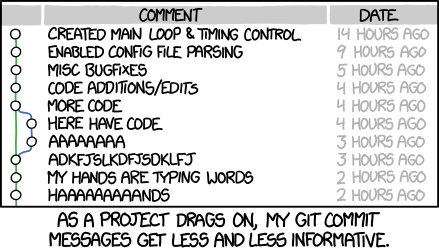
\includegraphics[width=0.6\linewidth]{images/xkcd_git_commit}\\
		{\tiny XKCD 1296, Randall Munroe}
	\end{center}
\end{frame}

\subsubsection{Bestanden negeren}
\begin{frame}[fragile]{Bestanden negeren}
	\begin{itemize}
		\item \texttt{git status} geeft onbekende bestanden altijd aan
		\item Oplossing: \texttt{.gitignore}:
	\end{itemize}
	\begin{minted}[bgcolor=light-gray]{text}
# alle bestanden in de map bin
bin/*

# alle .exe
*.exe

# maar wel dinges.exe
!dinges.exe
	\end{minted}

	(\texttt{.gitignore} moet wel gecommit worden)
\end{frame}

\begin{frame}{Bestanden alleen voor jezelf negeren}
	\texttt{.git/info/exclude}:
	\begin{itemize}
		\item Alleen op je eigen kopie van repo
		\item Zelfde syntax als \texttt{.gitignore}
	\end{itemize}

	Wat te negeren:
	\begin{itemize}
		\item Gegenereerde resultaten (binaries, logs)
		\item Gevoelige informatie (API keys, \ldots)
		\item Heel grote bestanden die veel veranderen (Github LFS)
	\end{itemize}
\end{frame}

\subsection{Geschiedenis bekijken}
% git log
\begin{frame}{log}
	\begin{tabularx}{\linewidth}{lX}
		\texttt{git log}
			& Bekijk geschiedenis van commits, standaard nieuwste boven (omkeren met \texttt{--reverse})\\
		\texttt{git log id1..id2}
			& Alle geschiedenis tussen \texttt{id1} en \texttt{id2}\\
		\texttt{git show}
			& Bekijk veranderingen in commit, standaard in nieuwste commit
	\end{tabularx}

	\medskip
	De ID's uit \texttt{log} kan je gebruiken in \texttt{git diff}:
\end{frame}

% git diff
\begin{frame}{git diff}
	\begin{tabularx}{\linewidth}{lX}
		\texttt{git diff}
			& Toon \textit{unstaged} veranderingen (niet ge\texttt{git add})\\
		\texttt{git diff --staged}
			& Toon veranderingen klaargezet voor commit\\
		\texttt{git diff HEAD\^}
			& Toon veranderingen sinds vorige commit\\
		\texttt{git diff id1 id2}
			& Toon verschil tussen commit \texttt{id1} en \texttt{id2}
	\end{tabularx}

	\medskip
	%{\footnotesize Waar je id's uit \texttt{git log} haalt. }
\end{frame}

% git show
\begin{frame}{git show}
	\begin{tabular}{l l}
		\texttt{git show}
			& Toon info over vorige commit\\
		\texttt{git show id}
			& Toon info over commit \texttt{id}\\
	\end{tabular}
\end{frame}

\subsection{Overzicht}
\begin{frame}{Overzicht (doemoment!)}
	{ \footnotesize
	\begin{tabular}{ll}
		\texttt{git init}						& maak een nieuwe repository \\
		\texttt{git status} 					& bekijk wat git denkt dat er aan de hand is \\
		\texttt{git add file1 [\ldots]}			& bestand(en) klaarzetten voor commit (stagen)	\\
		\texttt{git commit} 					& klaargezette bestanden in geschiedenis zetten (committen)\\
		\texttt{git reset file}		    		& bestanden ontstagen (omgekeerde van \texttt{add})	\\
		\hline
		\texttt{git diff}						& Veranderingen in aan Git bekende bestanden		\\
		\texttt{git diff --staged}				& Wat ga ik committen? (wat is staged?)				\\
		\texttt{git diff HEAD\^}				& Wat is er veranderd sinds de vorige commit?		\\
		\hline
		\texttt{git log}						& Bekijk vorige commits								\\
		\texttt{git show id}					& Bekijk commit \texttt{id} in detail
	\end{tabular}
	}
	{\small
	\begin{enumerate}
		\item \url{j.mp/gitgudslides}: download \texttt{simpelscript.sh} naar lege map
		\item Open Git Bash: \texttt{git init}; \texttt{git add}; \texttt{git commit}: eerste commit
		\item \texttt{bash simpelscript.sh}: runt programma
		\item Bug: 16 moet \texttt{`date +\%d`} zijn, repareer en commit \\
			(\texttt{`} is een backtick, linksboven op je toetsenbord)
		\item \texttt{bash simpelscript.sh}

		\item Probeer ook \texttt{git log}, \texttt{git show}
	\end{enumerate}
	}
\end{frame}

\section[Ongedaan]{Dingen ongedaan maken}

\subsection{Bestand terugdraaien naar onbewerkt}
\begin{frame}{Bestand terug naar vorige commit}
	\texttt{git checkout -- <bestand>} \\
	\alert{Omdat dit niet gecommit was ben je je wijzigingen kwijt!}
\end{frame}

\subsection{Bestanden terugdraaien naar eerdere versie}
\begin{frame}{Bestand(en) terug naar eerdere versie}
	\begin{itemize}
		\item \texttt{git checkout <hash> <bestand>}: enkele bestanden
		\item \texttt{git checkout HEAD <bestand>}
		\item \texttt{git checkout <hash>}: detached HEAD
		\item \texttt{git checkout master}: detached HEAD ongedaan maken
	\end{itemize}

	Allemaal veilig!
	%(Hash opzoeken met git log, of: \texttt{HEAD\^, HEAD\^\^, HEAD\textasciitilde 5})
\end{frame}

\begin{frame}{Detached HEAD in plaatjes}
	\begin{center}
		\includegraphics[width=.7\textwidth]{graphs/basis3.eps}<1,3>
		\includegraphics[width=.7\textwidth]{graphs/basis4.eps}<2>
	\end{center}
	\only<1>{Basisstaat van eerder}
	\only<2>{\texttt{git checkout B}}
	\only<3>{\texttt{git checkout master} (niet \texttt{C}!)}
\end{frame}

\subsection{Commits ongedaan maken}
\begin{frame}{git revert}
	\begin{itemize}
		\item \texttt{git revert <hash>}: maak nieuwe omgekeerde commit
		\item Safe: reverts van reverts van reverts kan je reverten
	\end{itemize}
\end{frame}

\begin{frame}{git reset}
	Veilig:
	\begin{itemize}
		\item \texttt{git reset}: unstage alles
		\item \texttt{git reset <bestand>}: unstage bestand
	\end{itemize}
	\alert{Onveilig:}
	\begin{itemize}
		\item \texttt{git reset --hard}: \texttt{checkout --} op hele working directory
		%\item \texttt{git reset <commit>}: verwijder alle commits na \texttt{<commit>}, laat WD staan
		%\item \texttt{git reset --hard <commit>}: \alert{dat is pech, data weg!}
	\end{itemize}
	%\alert{Reset alleen lokale dingen!}
\end{frame}

\begin{frame}{git clean}
	\alert{Verwijdert untracked bestanden!}
	\begin{itemize}
		\item \texttt{git clean -n}: dry run
		\item \texttt{git clean -x}: inclusief genegeerd
		\item \texttt{git clean -d}: untracked mappen
		\item \texttt{git clean --force}: \alert{poef}
	\end{itemize}
	(Soms beter om een snapshot van je branch te downloaden)
\end{frame}

\subsection{Overzicht}
\begin{frame}{Overzicht}
	{ \footnotesize
	\begin{tabular}{ll}
		\texttt{git checkout -- bestand}		& bestand terug naar vorige commit	\\
		\texttt{git commit} & klaargezette bestanden in geschiedenis zetten (committen)\\
		\texttt{git reset}	& bestanden ontstagen (omgekeerde van \texttt{add}
	\end{tabular}
	}
	Doen:
	\begin{enumerate}
		\item Ga terug naar je repo van eerder
		\item Run het script (\texttt{bash simpelscript.sh}) $\rightarrow$ untracked file
		\item \texttt{git clean -n}, \texttt{git clean -f}
		\item \texttt{bash simpelscript.sh}
		\item \texttt{.gitignore} maken met \texttt{laatstekeer.txt}, \texttt{git add .gitignore}
		\item \texttt{git clean -n} : bestand weg?
		\item \texttt{git clean -xn}, \texttt{git clean -xf}
		\item Commit je \texttt{.gitignore}
	\end{enumerate}
	Cheat sheet van eerdere dingen? \url{http://overapi.com/git}
\end{frame}

\section{Branching}

\subsection{Wat zijn branches?}
\begin{frame}
	\texttt{git status}: On branch master \ldots
\end{frame}

\begin{frame}{Wat is een branch?}
	\begin{itemize}
		\item Branch: verwijzing naar commit (die naar een commit verwijst, die naar \ldots)
		\item Manier om verschillende versies van je geschiedenis te hebben
	\end{itemize}
	Voorbeeld volgt
\end{frame}

\begin{frame}
	\begin{center}
		\only<1>{
			\includegraphics[width=.7\textwidth]{graphs/branching1.eps}
		}
		\only<2>{
			\includegraphics[width=.7\textwidth]{graphs/branching2.eps}
		}
		\only<3>{
			\includegraphics[width=.7\textwidth]{graphs/branching3.eps}
		}
		\only<4>{
			\includegraphics[width=.7\textwidth]{graphs/branching4.eps}
		}
		\only<5>{
			\includegraphics[width=.7\textwidth]{graphs/branching5.eps}
		}
		\only<6>{
			\includegraphics[width=.7\textwidth]{graphs/branching6.eps}
		}
		\only<7>{
			\includegraphics[width=.7\textwidth]{graphs/branching7.eps}
		}
		\only<8>{
			\includegraphics[width=.7\textwidth]{graphs/branching8.eps}
		}
		\only<9>{
			\includegraphics[width=.7\textwidth]{graphs/branching9.eps}
		}
	\end{center}
	\only<2>{
		\texttt{git branch feature}
	}
	\only<3>{
		\texttt{git checkout feature}
	}
	\only<4>{
		\ldots, \texttt{git commit}
	}
	\only<5>{
		\texttt{git checkout master}
	}
	\only<6>{
		\texttt{git checkout feature}, \ldots, \texttt{git commit}
	}
	\only<7>{
		\texttt{git checkout master; git merge feature}
	}
	\only<8>{
		\texttt{git checkout master}, \ldots, \texttt{git commit}
	}
	\only<9>{
		\texttt{git merge feature}
	}
\end{frame}

\subsection{Branches starten}
\begin{frame}{Branches starten}
	\begin{itemize}
		\item Standaard zit je op branch \texttt{master}
		\item Splits hiervanaf met \texttt{git branch <naam>}
		\item Splitsen van een eerdere commit:\\
			\texttt{git branch <naam> <hash>}
	\end{itemize}
\end{frame}

\begin{frame}{Branches wisselen}
	Na het maken van een branch moet je aangeven dat je op deze branch verder wil:
	\begin{itemize}
		\item \texttt{git checkout <naam>}
		\item \texttt{git checkout -b <naam>}: maak branch en switch direct
	\end{itemize}
	Hierna committen etc.
\end{frame}

\begin{frame}{Branches samenvoegen}
	\begin{enumerate}
		\item Switch naar branch waar je wijziging naartoe moet
		\item \texttt{git merge <naam>}
			\begin{itemize}
				\item Als base branch geen nieuwe commits heeft: fast-forward (commits worden direct overgenomen)
				\item Als wel: merge commit (2 parents), message typen
			\end{itemize}
	\end{enumerate}
\end{frame}

\subsection{Merge conflicts}
\begin{frame}[fragile]{Merge conflicts}
	Als zelfde gebieden in beide bestanden gewijzigd werkt het vorige niet gelijk:
	\begin{minted}[fontsize=\footnotesize,bgcolor=light-gray]{diff}
<<<<<<< HEAD
Aangepast na splitsing!
=======
Bestand aangepast van basisbranch
>>>>>>> dinges
	\end{minted}
	\begin{itemize}
		\item Handmatig bewerken (zie \texttt{git status})
		\item \texttt{git mergetool}
	\end{itemize}
	Wanneer opgelost: commit
\end{frame}

\subsection{Branch management}
\begin{frame}{Branch management}
	\begin{itemize}
		\item \texttt{git branch [-v]}: toon alle branches (en laatste commit)
		\item \texttt{git branch --no-merged}: wat is niet gemerged?
		\item \texttt{git branch -d naam}: verwijder (gemergede) branch
		%\item \texttt{git log --graph --all --oneline --decorate} Overzicht van geschiedenis:
	\end{itemize}
\end{frame}

\subsection{Branchen en workflows}
\begin{frame}{Workflows bij branchen}
	\alert{Beste optie: topic branches}
	\begin{itemize}
		\item Voor iedere feature een nieuwe branch, mergen wanneer klaar
		\item Je kan altijd \emph{gemakkelijk} terug naar voor je begon
		\item Je kan wijzigingen maken die nog niet helemaal werken / af zijn
		\item Base branch kan wijzigen (samenwerken!) zonder dat je in de problemen zit
	\end{itemize}
\end{frame}

\section{Samenwerken}

\subsection{Remotes}
\begin{frame}{Remotes}
	Remote: andere (volledige) git repo met gedeeld punt in geschiedenis
	\begin{itemize}
		\item \texttt{git remote -v}: toon remotes met url
		\item \texttt{git remote add <naam> <url>}: \texttt{naam} wordt alias voor \texttt{url}
	\end{itemize}
	Goede plekken om je repository te hosten:
	\begin{itemize}
		\item Github: veel gebruikt, Travis, gratis student account (private repo's beperkt)
		\item Bitbucket: alternatief voor Github, onbeperkt private repo's
		\item UU GitLab: intern voor de UU, mailinglijst, onbeperkt private repo's
	\end{itemize}
\end{frame}

\subsection{Bestaande repo overnemen}
\begin{frame}{git clone}
	Kopieer repository en maak remote `origin'
	\begin{itemize}
		\item \texttt{git clone <url>}
		\item \texttt{git clone <url> <map>}
	\end{itemize}
	Als niet je eigen repo en wel toevoegingen maken: forken
\end{frame}

\subsection{Wijzigingen binnenhalen}
\begin{frame}{git fetch}
	\begin{itemize}
		\item Kopieer commits van een remote naar je repo
		\item Je krijgt ze nog niet direct zichtbaar, maar als remote branch:
		\item \texttt{git diff origin/branch} toont wat nieuw is
		\item \texttt{git merge origin/branch} neemt de (wijzigingen in de) commits over
		\item \texttt{git pull} : \texttt{fetch} + \texttt{merge} ineen
		\item Zorg voor een schone working directory!
	\end{itemize}
\end{frame}

\subsection{Wijzigingen publiceren}
\begin{frame}{git push}
	\begin{itemize}
		\item Kopieer commits van je repo naar een remote
		\item Vergelijkbaar met een pull vanaf je remote
		\item Wanneer nieuwe branch: \texttt{git push --set-upstream origin branch}
	\end{itemize}
\end{frame}

\subsection{Pull requests}
\begin{frame}{Pull requests}
	\begin{itemize}
		\item Geen echt git-mechanisme
		\item ``Hee, wil jij \texttt{git pull blabla} doen?''
		\item Kom je veel tegen in Github etc.
	\end{itemize}
\end{frame}

\begin{frame}{Overzicht}
	\begin{tabular}{ll}
		\texttt{git remote}		& Beheer servers waar je vandaan/naar pusht\\
		\texttt{git clone}		& Maak een lokale kopie van een repo\\
		\texttt{git fetch}		& Download wijzigingen, maar hou ze apart (te mergen)\\
		\texttt{git pull}		& Fetch en merge gelijk\\
		\texttt{git push}		& Kopieer commits naar remote
	\end{tabular}
	Doen:
	\begin{enumerate}
		\item Ga naar een niet-repo map
		\item Open \url{https://j.mp/gitgud-repo}, maak account, fork
		\item Clone je geforkte repo
		\item Zet je naam of iets anders op de lijst
		\item Commit, push, pull request via de site
	\end{enumerate}
\end{frame}

\section[Hoe verder?]{Hoe verder na deze tutorial?}

\begin{frame}{Mogelijkheden}
	Git heeft heel veel mogelijkheden voor verschillende use-cases:
	\begin{center}
		\begin{tabular}{ll}
			\texttt{alias} & Verkort veelgebruikte commando's \\
			\texttt{grep}	& Doorzoek alle bij Git bekende bestanden \\
			\texttt{submodules} & Sluit een ander volledig git-repository in \\
			\texttt{stash} & Sla wijzigingen tijdelijk op\\
			Hooks & Voer scripts uit wanneer je iets doet in Git \\
			Travis CI & Bouw en publiceer iets bij elke \texttt{git push}
		\end{tabular}
	\end{center}
	Lees de handleiding: \texttt{git help [commando]}
\end{frame}

\begin{frame}{Extra hulpbronnen}
	\begin{itemize}
		\item Pro Git, het offici\"ele boek: \url{https://git-scm.com/book}
		\item Interactieve tutorials:
			\begin{itemize}
				\item \url{https://try.github.io}
				\item \url{https://codecademy.com/learn/learn-git}
			\end{itemize}
		\item \url{https://www.atlassian.com/git/tutorials/}
		\item \emph{Google} en zelf doen!
	\end{itemize}
\end{frame}

\begin{frame}{git alias}
	Maak verkortingen voor commando's:
	\begin{itemize}
		\item \texttt{git config alias.overzicht "log --all --graph --decorate --oneline"}
		\item \texttt{git config alias.unstage "reset HEAD"}
	\end{itemize}
	Maak aliases global (voor al je git repo's op die computer) met \texttt{git config --global \ldots}
\end{frame}

\begin{frame}{git grep}
	Zoeken in alle tracked files:
	\begin{itemize}
		\item \texttt{git grep "Zoeken"}
		\item \texttt{git grep -i "zOEkEn"} hoofdletterongevoelig
		\item \texttt{git grep -n "Zoeken"} regelnummer
		\item \texttt{git config --global alias.zoek "grep -ni"} alias voor beide
	\end{itemize}
\end{frame}

\begin{frame}{Dat was het dan}
	De slides zijn op
\end{frame}


\end{document}
